\section{Ergebnisse und Diskussion}
\label{sec-6}
\begin{comment}
\fbox{
\parbox{\linewidth}{
\textit{Ziel des Kapitels:}\\
Ergebnisse der Umsetzung vorstellen und auf die Fragestellung anwenden.
}}
\end{comment}

Ziel dieser Arbeit war es, zu untersuchen, wie ein konkretes physikalisches Experiment durch eine Anwendung mit der HoloLens unterstützt werden kann. Dafür wurde ein Versuch aus der Elektrodynamik ausgewählt, Probleme identifiziert und eine Lösung erarbeitet. Diese soll nun im Hinblick auf die in der Problemstellung festgehaltenen Anforderungen bewertet werden. Die Ergebnisse werden dann im breiteren Kontext der Fragestellung diskutiert.

\begin{comment}

\begin{itemize}
\item Welche physikalischen Zusammenhänge werden vermittelt?
\item Wie 
\end{itemize}

Konkrete untergeordnete Frage:
\begin{center}
\textit{\textbf{Wie kann die HoloLens in einem konkreten Anwendungsfall eines physikalischen Versuches genutzt werden?}}
\end{center}
\subsection{Aufgabenstellung}

Im Rahmen der Arbeit soll anhand der HoloLens untersucht werden, wie diese in der Physik-Lehre eingesetzt werden kann, um physikalische Inhalte zu vermitteln. Insbesondere soll betrachtet werden, wie physikalische Experimente mittels Mixed Reality Anwendungen durch zusätzliche Inhalte angereichert werden können.\\

\par
Dazu sind zunächst die technischen Möglichkeiten und Voraussetzungen der HoloLens zu betrachten und in Zusammenhang mit dem Anwendungsfall zu bringen. Weiterhin sind bestehende Ansätze im Einsatz von Mixed Reality Technologie in der Lehre, besonders in der Physik-Lehre, herauszuarbeiten und einzuordnen.

Davon ausgehend soll der Fragestellung anhand eines konkreten Beispiels nachgegangen werden. Für einen ausgewählten Versuchsaufbau sind die darzustellenden Objekte und Informationen sowie das Zusammenspiel dieser mit dem aufgebauten Experiment, der Umgebung und den Nutzern zu entwickeln. Für den ausgewählten Anwendungsfall soll eine Umsetzung mit der HoloLens konzipiert, designet und prototypisch implementiert werden.
\end{comment}

\subsection{Ergebnisse}
 Die Lösung integriert virtuelle Elemente in das Experiment, die relevante, physikalische Zusammenhänge abbilden. Dazu gehören interaktive Darstellungen des Magnetfeldes sowie Messwerte, der Stromfluss und ein Kompass. Durch eine dreidimensionale Einbettung in den tatsächlichen Versuchsaufbau wird ein direkter Zusammenhang zwischen dem Verhalten der Objekte des Versuches und den physikalischen Modellen hergestellt.
 \par
 \noindent\hspace*{5mm}
 Gleichzeitig berücksichtigt das Design die besonderen technischen Modalitäten der HoloLens. Auf der einen Seite wird von den verschiedenen technischen Möglichkeiten Gebrauch gemacht (Tracking, World Anchor, stereoskopisches see-through Display, Gestenerkennung, etc.). Auf der andern Seite werden technisch bedingte Anforderungen an das Design von Anwendungen berücksichtigt (Abstand, Größe, Farbe, Positionierung, Performance, etc.).
 \par
 \noindent\hspace*{5mm}
 Im Weiteren sollen die Ergebnisse zunächst aus anwendungsorientierter Sicht näher vorgestellt werden, bevor auf die Resultate aus technischer Sicht eingegangen wird.
 
\subsubsection{Unterstützung des Experimentes}
Die Anwendung unterstützt die Vermittlung der physikalischen Zusammenhänge durch die Integration der entsprechenden Modelle und Darstellungen in den Versuchsaufbau und -Ablauf. Im Wesentlichen umfasst die Lösung diesbezüglich folgende, inhaltliche Funktionen:
\vspace{8px}
\begin{center}
	\fbox{
		\parbox{0.9\linewidth}{
			\vspace{4px}
			\textit{Unterstützung des Versuches}
			\begin{itemize}[rightmargin=12px, topsep=-12px]
				\setlength{\itemsep}{-1pt}
				\singlespacing
				\item Visualisierung der Komponenten des Magnetfeldes in zwei Darstellungen und in Echtzeit
				\item Darstellung einer vorberechneten, numerischen Lösung für eine ausgewählte Ebene des Feldes der Spule
				\item Kennzeichnung des Stromflusses
				\item Integration eines Kompass mit Hervorhebung wichtiger Zustände
				\item Einbettung einer virtuellen Kompassnadel auf Basis theoretischer Werte
				\item Numerische Darstellung gemessener und berechneter Echtzeitdaten
			\end{itemize}
			\vspace{18px}
	}}\\
\end{center}
\vspace{6px}

Durch den gewählten Designansatz werden die physikalischen Eigenschaften in ihrem realen, räumlichen und zeitlichen Kontext dargestellt. Somit kann ein direkter Zusammenhang zwischen dem Verhalten der Objekte des Versuches und den physikalischen Modellen, Darstellungen und Messwerten hergestellt werden. Dabei unterstützt die Anwendung in erster Linie ein qualitatives Verständnis. Die durch die Applikation gestützten Zusammenhänge lassen sich wie folgt zusammenfassen:

\vspace{8px}
\begin{center}
	\fbox{
		\parbox{0.9\linewidth}{
			\vspace{4px}
			\textit{Physikalische Zusammenhänge}
			\begin{itemize}[rightmargin=12px, topsep=-12px]
				\setlength{\itemsep}{-1pt}
				\singlespacing
				\item Räumliches Verständnis des Feldes der Spule
				\item Zusammenhang zwischen Stromstärke und Flussdichte
				\item Verständnis der verschiedenen Darstellungsmodelle
				\item Zusammenspiel der Einzelfelder von Erde und Spule
				\item Auswirkungen des entstehenden Feldes auf die Magnetnadel
				\item Einfluss von Störfaktoren wie Reibung und Trägheit auf die Nadel
			\end{itemize}
			\vspace{18px}
	}}\\
\end{center}
\vspace{6px}

\textit{Feld der Spule}\\
Die verschiedenen Darstellungen geben zusammen einen Einblick in die Struktur des dreidimensionalen Feldes der Spule. Die Richtung, Stärke und Homogenität des Feldes werden für das Innere der Spule in Echtzeit dargestellt. In der Vektordarstellung wird auch das dreidimensionale, inhomogene Feld angedeutet. Einen Eindruck von der Struktur des gesamten Feldes gibt die Darstellung der numerischen Lösung. Hier ist zwar zunächst nur eine Ebene dargestellt, allerdings ist diese repräsentativ für den gesamten Raum, da das Feld symmetrisch ist.\\

\textit{Stromstärke und Flussdichte}\\
Die lineare Abhängigkeit zwischen Stromstärke und Flussdichte wird durch die Interaktion mit der Spannungsquelle deutlich. Eine gleichmäßige Änderung des Reglers hat eine gleichmäßige Änderung der Darstellungen zu Folge, ohne wahrnehmbare zeitliche Verzögerung. Der Nutzer kann hier folglich selbstständig das System mit beiden Darstellungsmodellen erforschen und den Zusammenhang erfahren.

\textit{Darstellungsmodelle}\\
Der Nutzer hat die Freiheit zwischen den Darstellungen des Magnetfeldes zu wechseln. In Zusammenhang mit der Möglichkeit, das zugrundeliegende Feld zu verändern, können so die unterschiedlichen Eigenschaften der Modelle erforscht werden.\\

\textit{Zusammenspiel der Einzelfelder und Auswirkung auf die Nadel}\\


\textit{Einfluss von Störfaktoren}\\
Die reale Magnetnadel unterliegt den Einflüssen von Reibung und Trägheit. Durch die eingebettete, theoretische Ausrichtung wird der Unterschied zwischen der realen und einer von Störeinflüssen freien Nadel deutlich.

\textit{Zusammenfassung}\\
Diese physikalischen Zusammenhänge sind am Versuchsaufbau allein so nicht ersichtlich und werden erst durch die Mixed-Reality Anwendung erkennbar.\\


Die Anwendung integriert alle in den Anforderungen festgehaltenen Elemente, bis auf die als optional eingestuften, weiteren Parameter des Experimentes. Wie die Lösung sicherstellt, dass die notwendigen Informationen auch tatsächlich erkennbar sind, ist in den einzelnen Umsetzungen gezielt erörtert.\\

\textbf{Bewertung anhand der Nicht-funktionale Anforderungen}\\
\textit{Korrektheit und Interpretierbarkeit}\\
Die Korrektheit und Interpretierbarkeit wird weitestgehend über die Nutzung etablierter physikalischer Darstellungsmodelle gesichert. Dabei liegt der Fokus nicht auf möglichst exakten Darstellungen numerischer Werte, sondern auf einer zweckmäßigen Darstellung. Im Vordergrund steht das qualitative Verständnis.\\

Die Anwendung ist jedoch nicht vollständig selbsterklärend, sondern bedarf einer Anleitung durch eine fachkundige Person. Das betrifft auch den Bereich Interpretierbarkeit in den Punkten:
\begin{itemize}
	\setlength{\itemsep}{-1pt}
	\singlespacing
	\item Räumliche Begrenzungen aller Felddarstellungen
	\item Einordnung der berechneten Vektoren und Feldlinien als Komponenten des resultierenden Feldes
	\item Einordnung der Simulationsdarstellung als unabhängig, vorberechnet und nur für die Spule allein zutreffend (ohne Feld der Erde)
	\item Einordnung der Darstellungen als approximativ
\end{itemize}

Die betroffenen Eigenschaften lassen sich zwar erahnen oder indirekt ableiten, werden jedoch nicht direkt durch die Applikation kommuniziert. Dafür könnte die Anwendung um eine Einführung z.B. durch einen eingesprochenen Text mit einer eigenen Sequenz entwickelt werden.\\

TODO: Abschnitt erweitern...

\textit{Weitere Aspekte}\\
Der Nutzer wird durch das Tragen der HoloLens nicht wesentlich in der Interaktion mit den Gerätschaften eingeschränkt. Alle wichtigen Elemente (Anschlüsse, Spannungsquelle, Kompassnadel, Messgeräte, Spule) bleiben sichtbar und werden wenn dann nur zu kleinen Teilen überblendet. Die Hände bleiben frei zum Einstellen der Geräte oder auch Aufschreiben von Notizen. Der Klicker hat eine kleine Schlaufe, so dass er nicht unbedingt festgehalten werden muss.\\

Die Applikation ist auch für Anwender ohne Erfahrungen mit der HoloLens oder Mixed Reality im Allgemeinen nutzbar, es müssen keine Handgesten erlernt werden. Allerdings kann die Nutzererfahrung bei unerfahrenen Nutzern durch ungünstige (z.B. hektische) Kopfbewegungen beeinträchtigt werden. Außerdem wurden die vorhandenen Gerätschaften genutzt.\\

TODO: Abschnitt erweitern...

\subsubsection{Technische Umsetzung}
Im Hinblick auf die technischen Anforderungen wurde eine Liste von Qualitätskriterien zugrunde gelegt. Die Bewertung der Lösung anhand dieses Maßstabes ist Tabelle \ref{tab:tech_results} zu entnehmen. Der Einschätzung liegen die zu jedem Kriterium genannten Hinweise zur Bewertung zu Grunde.
%\textbf{Qualitätskriterien}
%\begin{sidewaystable}[h!]
\begin{landscape}
	\bgroup
	\setlength\extrarowheight{-2pt}
	\def\arraystretch{1.8}
	\begin{table}
		\centering
		\begin{tabular}{m{2.3cm}|m{15.5cm}|m{2cm}}
			Kriterium & Ergebnis & Bewertung\\
			\hline
			\hline
			Framerate & Durchgehend 60 FPS, keine Framedrops. Einzig bei Start/Stopp von Vuforia hängt die Anwendung kurz (<1s). & Optimal\\
			\hline
			Stabilität der Hologramme & Hologramme erscheinen durchgehend sehr stabil, Elemente liegen im Abstand von max. 20cm zu einem Spatial Anchor und der Stabilization Plane. Seltene, minimale Sprünge sowie Wippen der simulierten Feldlinien treten auf. Objekte, die sehr dicht an realen liegen, driften bei Bewegungen leicht & Fast optimal\\
			\hline
			Positionierung & Sehr genaue Positionierung über optischen Marker. Hologramme sind glaubhaft in die Spule eingebettet. Überschneidungen von wenigen Millimetern sind jedoch möglich. & Fast optimal\\
			\hline
			Komfortzone & Elemente liegen in Komfortzone (Winkel und Distanz), sofern eine geeignete Unterlage vorhanden ist. Design begünstigt den gewünschten Abstand. Minimale Distanz wird über Fading sichergestellt. & Optimal\\
			\hline
			Fokuswechsel & Kaum Neufokussierungen notwendig. Nur bei Ablesen des Kompass und der Stromrichtung. & Fast optimal\\
			\hline
			FOV-Grenzen & Darstellungen passen bei empfohlener Distanz vollständig in FOV. Durch Verankerung am realen Objekt verliert Nutzer den Kontext nicht. & Optimal\\
			\hline
			Anpassung an Nutzerposition & Text, Labels, Linien und Menüs richten sich zur Nutzerposition aus. Frei bewegliche Elemente (Menü, Progress Indikator) folgen Nutzer. & Optimal\\
			\hline
			Input Interaction Clarity & Vorhandene, einfache Standard-Interaktionsmechanismen genutzt und geringfügig erweitert. Konsistentes, akustisches Feedback. Jedoch keine Erklärung der möglichen Aktionen durch die Anwendung selbst. & Mittel\\
			\hline
			Interaktive Objekte & Vorhandene Buttons, Felder und Cursor genutzt. & Optimal\\
			\hline
			Ladevorgänge & Vorhandenen, animierten Progress Indikator verwendet. Lesbarkeit des Textes wird abgesichert. Vorgänge sind kurz, keine Angabe einer erwarteten Dauer notwendig. & Optimal\\
		\end{tabular}\caption{\label{tab:tech_results} Bewertung der Umsetzung anhand von Qualitätskriterien.}
	\end{table}
	\egroup
%\end{sidewaystable}
\end{landscape}

Insgesamt erfüllt die Applikation die Anforderungen fast vollständig bis vollständig. Einige Probleme konnten bereits im Design abgemildert oder umgangen werden. Das gilt z.B. für die Aspekte Komfortzone und FOV-Grenzen. Durch die platzsparende Anordnung der Elemente werden die Hologramme seltener abgeschnitten. Außerdem sind häufige Kopfbewegungen und Hinweise auf Elemente außerhalb des FOV so nicht notwendig. Und die Berücksichtigung einer geeigneten Distanz von Beginn an vermeidet bzw. verringert Probleme mit zu dicht positionierten Objekten.\\

Die Umsetzung unterstützt bereits im Design verankerte Maßnahmen weiter. Hier wurde z.B. bei der Festsetzung von Anzahl und Größe von Objekten auf die Einschränkungen der HoloLens Rücksicht genommen. Viele Probleme werden auch durch die Nutzung von vorgefertigten Objekten und Verhaltensweisen vermieden. Hier sind z.B. der Progress Indikator, Standard-Button und Standard-Shader zu nennen. Im Weiteren soll auf einzelne Aspekte kurz näher eingegangen werden.\\

\textit{Field of View}\\
Die Darstellungen passen bei einer üblichen Position vollständig in die Grenzen des Sichtfeldes. Der Screenshot in Abb. \ref{img:fov} zeigt die Kameraperspektive aus solch einer Position. Dabei ließe sich der Kopf horizontal in beide Richtungen etwa 6° drehen, ohne dass die Hologramme abgeschnitten werden würden.
\begin{wrapfigure}{r}{0.5\textwidth}
	\centering
	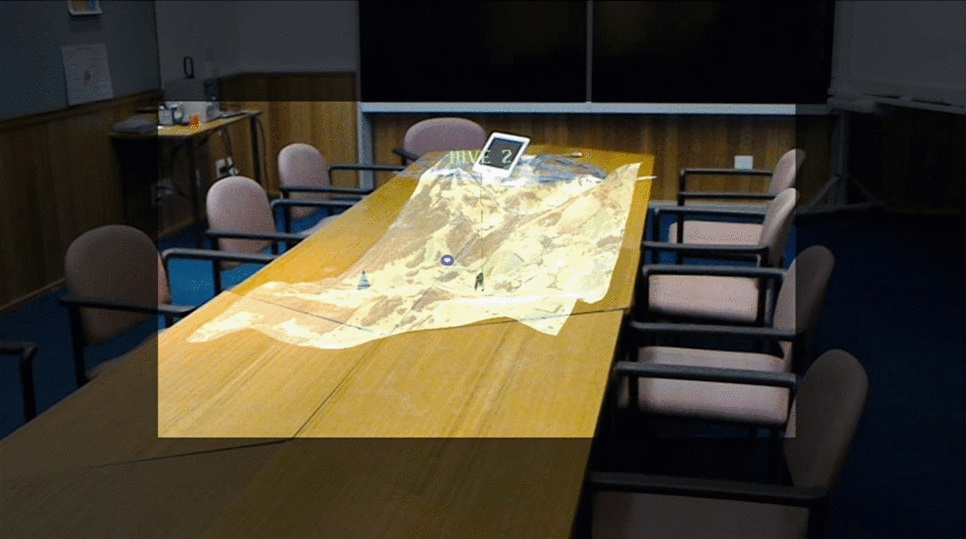
\includegraphics[width=0.48\textwidth]{images/unity/fov.jpg}
	\caption{Screenshot zeigt Kameraperspektive bei 1,5m Distanz zum Zentrum der Spule, 30° Neigung. Auflösung und Seitenverhältnis entspricht dem eines einzelnen Displays auf der HoloLens.}
	\label{img:fov}
\end{wrapfigure}

\textit{Stabilität}\\
Die Stabilität der Objekte beeinflusst die Nutzererfahrung wesentlich, da durch die Einbettung in die Spule selbst geringe Abweichungen negativ auffallen. Bei einer umsichtigen Nutzung treten diesbezüglich wenige bis keine Probleme auf, die Elemente wirken stabil. Lediglich die sehr nah an der Spule positionierten Daten-Panels und Tooltips können bei Bewegungen einen leichten Drift aufweisen. Selten sind kleinere Sprünge oder Vibrationen festzustellen. Und die Darstellung der Feldlinien wippt bei vertikalen Kopfbewegungen leicht um den Mittelpunkt. Das ist der Tatsache geschuldet, dass die Feldlinien steil auf der Stabilisations-Ebene stehen und sich von dieser bis zu 1,2 Meter ausbreiten. Der Effekt ist jedoch gering und nur auffällig, wenn er provoziert wird.\\

Allerdings hängt die Stabilität nicht unwesentlich von den Randbedingungen ab. Die weiter unten genannten Umstände des Tests erleichtern das Tracking und die Stabilisation. Unter weniger geeigneten Bedingungen kann die Stabilität und damit auch die Positionierung der Hologramme beeinträchtigt werden. Insbesondere kann es bei unerfahrenen Nutzern durch ungünstige Aktionen wie z.B. ruckartige Kopfbewegungen zu negativen Auswirkungen auf die Stabilität kommen.\\

\textit{Positionierung}
\begin{wrapfigure}{r}{0.5\textwidth}
	\centering
	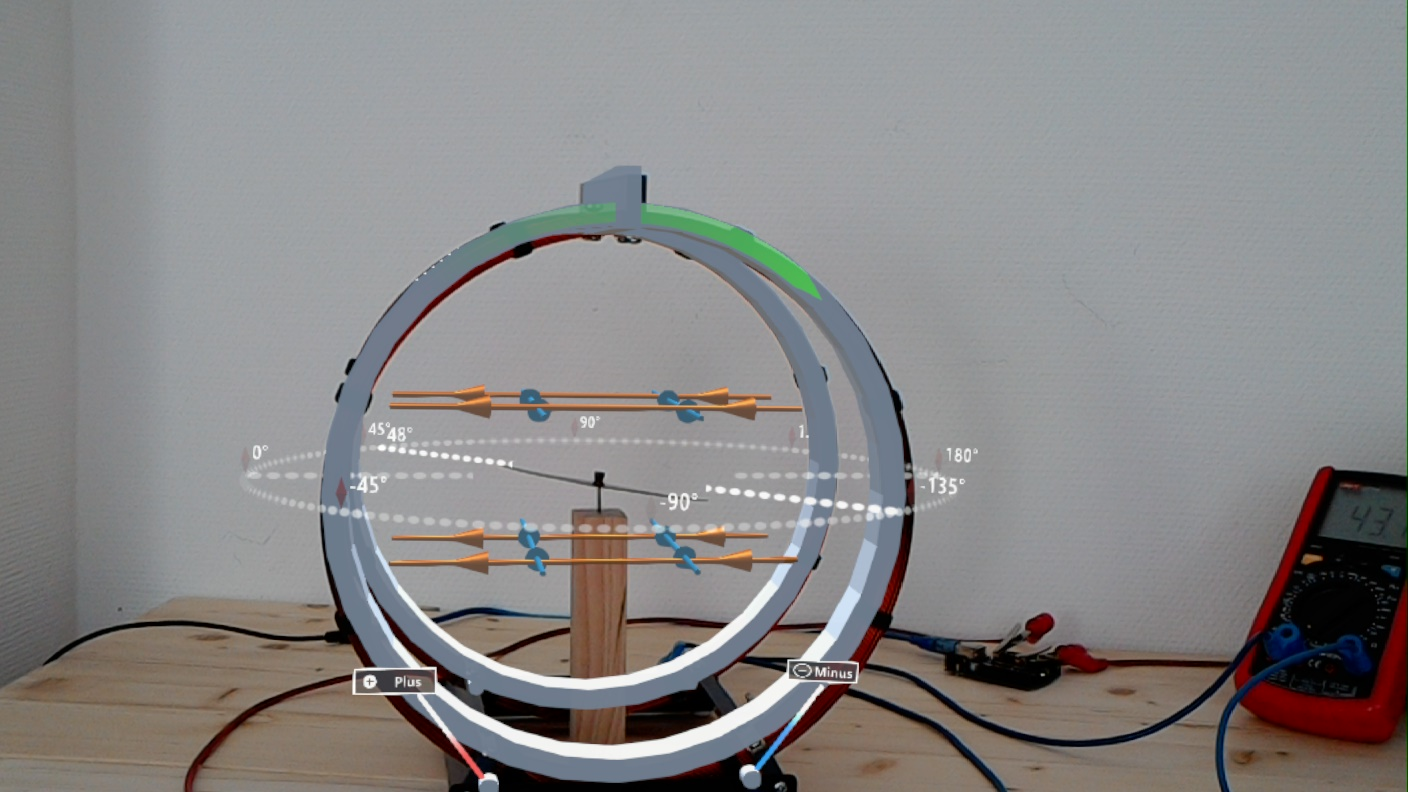
\includegraphics[width=0.48\textwidth]{images/HL/model-overlay.jpg}
	\caption{Überlagerung virtuelle und reale Spule}
	\label{img:model-overlay}
\end{wrapfigure}
Einen Eindruck von der Güte der Positionierung lässt sich anhand von Abb. \ref{img:model-overlay} gewinnen. Das normalerweise nur in den Tiefenpuffer gerenderte Mesh der virtuellen Spule wird hier durch einen Standard-Shader sichtbar dargestellt. Die reale Spule ist dadurch fast gar nicht zu sehen. Zwar sind Abweichungen zwischen den beiden Objekten aus unterschiedlichen Winkeln unterschiedlich stark sichtbar, das gewählte Foto gibt jedoch einen guten Anhaltspunkt für die tatsächliche Nutzererfahrung wieder.\\

\textit{Interaction Clarity}\\
In Puncto Interaction Clarity kann die Lösung nur als mittel eingestuft werden. Denn das Kriterium verlangt ausdrücklich, dass eine Anwendung die ihr zu Grunde liegenden Interaktionsmöglichkeiten erklärt, sofern sie über Gewohntes hinausgehen. Das ist hier bei der Steuerung außerhalb des Menüs nicht der Fall. Die Lösung setzt eine Anleitung durch eine begleitende Person voraus, die den Anwender über die möglichen Aktionen informiert. Die anderen Punkte des Kriteriums werden jedoch erfüllt.\\

\textit{Performance}\\
Etwas ausführlicher soll hier noch der Ressourcenverbrauch der Applikation beleuchtet werden. Die Performance hat maßgeblichen Einfluss auf die Stabilität und Positionierung der Hologramme und ist daher besonders wichtig. Die Anwendung wurde mit Hilfe von Unity's Profiler sowie des Windows Performance Analyzers bei einem ein-minütigem Einsatz auf der HoloLens analysiert. Dabei wurde das Menü und die drei verschiedenen Darstellungen aufgerufen.

\begin{figure}[h!]
	\centering
	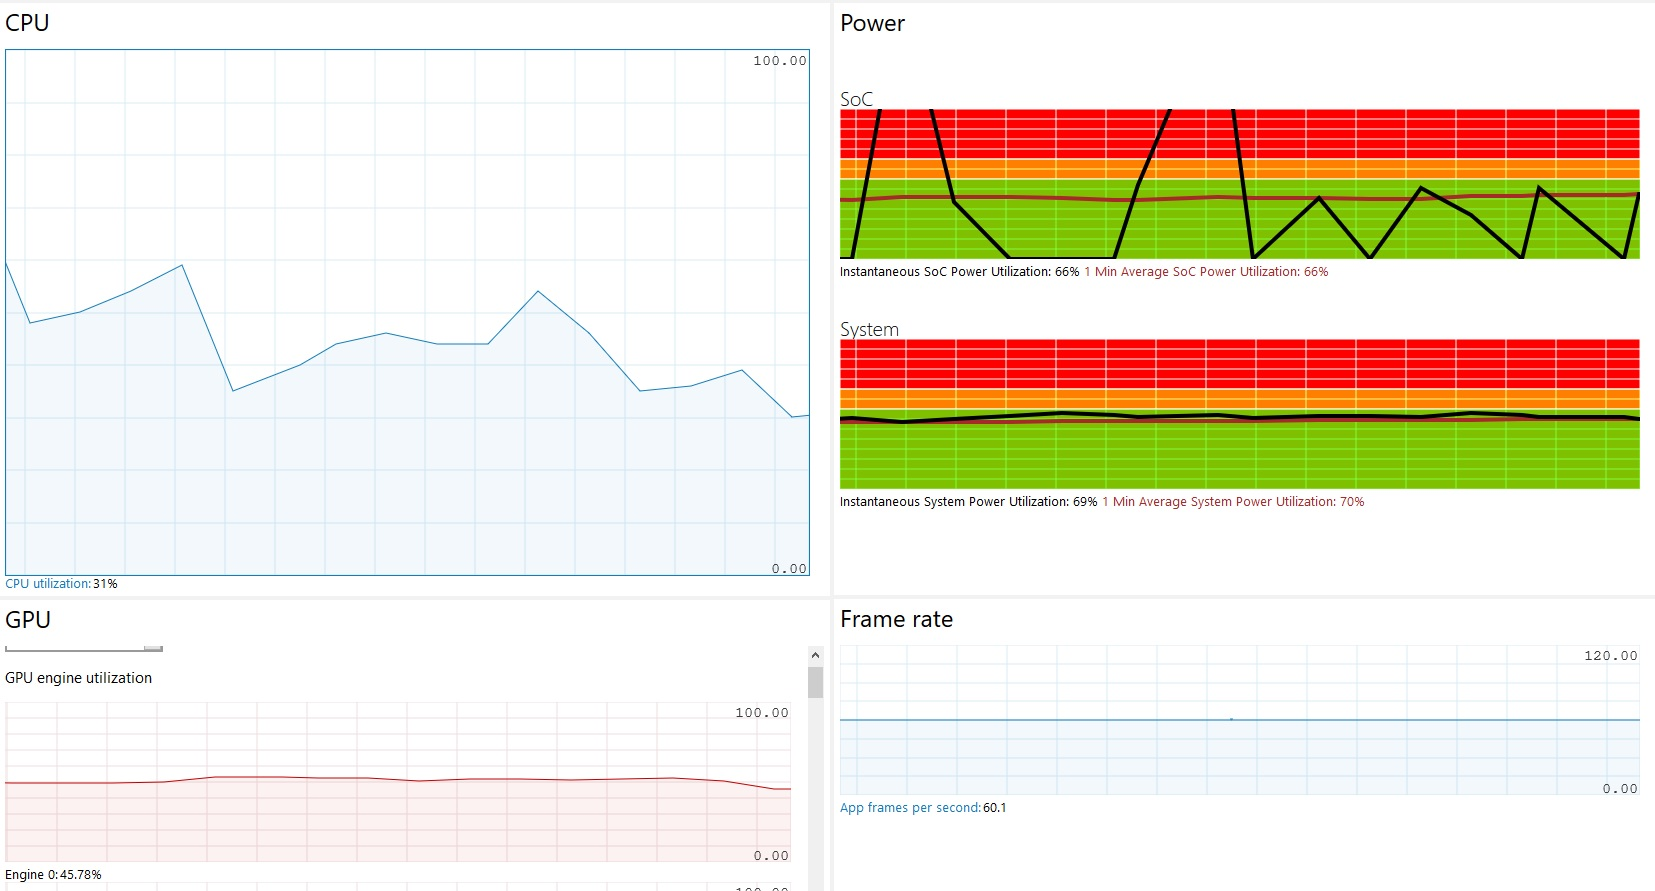
\includegraphics[width=\textwidth]{images/performance/performance.jpg}
	\caption{Performance Monitor}
	\label{img:performance}
\end{figure}

Einen Eindruck vom Ressourcenverbauch der App vermittelt der Screenshot in Abb. \ref{img:performance}. Zu sehen ist die Auslastung der Brille über einen Zeitraum von 60 Sekunden. Währenddessen wurde mehrfach zwischen den verschiedenen Darstellungen hin- und hergewechselt und das Menü aufgerufen.

\begin{figure}[h!]
	\centering
	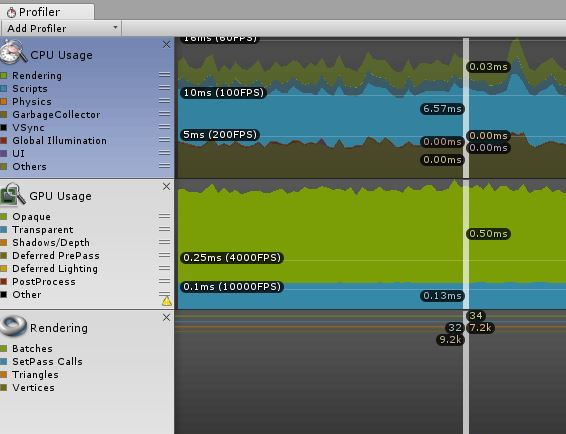
\includegraphics[width=\textwidth]{images/performance/profiler.png}
	\caption{Profiler}
	\label{img:profiler}
\end{figure}

\begin{itemize}
	\setlength{\itemsep}{-1pt}
	\singlespacing
	\item Konstante Framerate von 60 FPS
	\item CPU: 60-30\% Auslastung
	\item GPU: 40-50\% Auslastung
	\item Stromverbrauch unregelmäßig
\end{itemize}

Insgesamt ist die Auslastung der Hardware relativ hoch. Zwar liegen sowohl bei CPU als auch GPU noch Reserven, allerdings bestimmt das Zusammenspiel von CPU und GPU die Framerate.\\

MSAA treibt Ressourcenverbrauch in die Höhe: ohne MSAA etwa 25\% GPU\\
Rendering der Linien besonders CPU-intensiv. knapp 7 ms CPU-Zeit nur für die Linien, ohne Optimierungen etwa 45 ms\\

\textit{Testbedingungen}\\
Die Bewertung wurde anhand von Tests unter für die Anwendung günstigen Bedingungen durchgeführt. Der Versuchsaufbau wurde so positioniert, dass die umliegenden Objekte gut für das Tracking der Brille geeignet sind. Außerdem wurde die HoloLens vorher öfter im Testraum verwendet und hatte daher bereits ein gutes Modell des Raums zur Orientierung. Weiterhin wurde die Brille auf den Tester kalibriert und ruckartige oder unnötige Kopfbewegungen vermieden. 

\subsubsection{Feedback}
Zur Bewertung der vorgestellten Lösung wurde die Anwendung außerdem unterschiedlichen Personen vorgestellt und zum Testen überlassen. Dabei handelt es sich um ca. 15 Personen mit unterschiedlichem Grad an Expertise. Das Spektrum umfasst ungefähr zu gleichen Teilen Akademiker, Lehrer und Studenten der Physik. Deren Feedback wurde für diese Arbeit qualitativ festgehalten und zusammengefasst. Die Nutzung der Anwendung beschränkte sich dabei meistens auf den Hauptteil mit den physikalischen Darstellungen.\\

\vspace{8px}
\begin{center}
	\fbox{
		\parbox{0.9\linewidth}{
			\vspace{4px}
			\textit{Qualitatives Feedback}
			\begin{itemize}[rightmargin=12px, topsep=-12px]
				\setlength{\itemsep}{-1pt}
				\singlespacing
				\item Insgesamt positive Bewertung aller Nutzer
				\item Besonders viel positives Feedback zu: 
				\begin{itemize}[topsep=-0.25em]
					\setlength{\itemsep}{-0.25em}
					\item Darstellung der numerischen Lösung 
					\item Interaktivität in Echtzeit
				\end{itemize}
				\item Häufig gewählte Wörter zur Beschreibung der Nutzererfahrung: ''Toll'', ''Cool'' und ''Beeindruckend''
				\item Fragen nach einer berechneten Darstellung für 3D
				\item Keine negativen Äußerungen zur Stabilität und Positionierung
				\item Anmerkungen zu hohem Aufwand und Praktikabilität
				\item Viele wollten gern Fotos der Anwendung haben
				\item Kaum Feedback von Lernenden, fast allen Nutzern waren die physikalischen Zusammenhänge bereits zu großen Teilen bekannt
			\end{itemize}
			\vspace{18px}
	}}\\
\end{center}
\vspace{6px}

\textit{Erfahrungen zur praktischen Nutzung der HoloLens}\\
Die Reaktionen lassen sich durchweg als positiv beschreiben. Obwohl die meisten Tester keine oder kaum Erfahrung mit der HoloLens oder anderen HMDs hatten, beschränkten sich die Schwierigkeiten in der Nutzung auf ein Minimum. Diese betrafen vor allem das Aufsetzen der Brille. Denn wenn diese nicht richtig sitzt, ist das ohnehin schon kleine Sichtfeld nicht vollständig sichtbar. Hier schaffte jedoch eine kurze Erklärung dazu, wie die Brille sitzen sollte, Abhilfe. Außerdem war die Klick-Geste für viele Nutzer nicht auf Anhieb nutzbar, deshalb wurde meist der Klicker bevorzugt. Die Limitierung des Sichtfeldes wurde nur vereinzelt negativ angemerkt.\\

Die Tatsache, dass größtenteils keine vorangegangenen Erfahrungen mit dem Nutzererlebnis der HoloLens bestanden, trägt natürlich nicht unwesentlich zu den oben genannten Reaktionen bei.\\

\subsection{Diskussion}
TODO...

Frage: Wie HoloLens einsetzen?

\begin{itemize}
	\item Über 3D-Darstellungen Felder im Raum anzeigen, profitiert von stereoskopischer Wahrnehmung und See-Through-Displays
	\item Empfohlene Verhaltensweisen durch Nutzung von vorgefertigten Elementen einbinden
	\item Interaktion einfach halten, z.B. durch Klicker
	\item Zusammenspiel von realen und virtuellen Objekten nutzen, nicht für alles muss eine softwareseitige Lösung geschaffen werden
	\item Virtuelle Objekte an Versuchsaufbau verankern, dadurch verliert Nutzer sie nicht
	\item Tracking der HoloLens nutzen, um Objekte zu positionieren, anstelle eines dauerhaft sichtbaren Markers, Stabilität ausreichend, dabei aber mögliche Störfaktoren beachten...
	\item ... Stabilität bei diesem Ansatz wichtig, daher Performance sehr wichtig, unbedingt beachten und Optimierungen vornehmen
	\item World Anchor kann für grobe Positionierung genutzt werden, um Setup-Zeit zu verringern
	\item Anwendung ist hochgradig zugeschnitten auf die konkreten Eigenschaften des Experimentes
	\item Einsatz per Streaming denkbar, dann jedoch weitere perf. Opt. notwendig oder Deaktivieren von MSAA
\end{itemize}


\subsubsection{Erweiterbarkeit}
Mögliche Erweiterungen:
\begin{itemize}
	\item Vorberechnete Feldlinien für ein 3D-Ausschnitt möglich
	\item Weitere Lehrinhalte denkbar: z.B. Entstehung und Überlagerung der Einzelfelder, Elektrisches Feld um die Leiter herum, Anderer Versuch: Ablenkung eines Elektronenstrahls in der Spule
	\item Applikation ist parametrisiert: Andere physikalische Parameter möglich
	\item Kaum noch Reserven für mehr Darstellungen, weitere perf. Opt. vornehmen, z.B. selektives Aktivieren/Deaktivieren von MSAA
	\item Variation von Spulengröße möglich, aber Anpassung der Parameter für die Darstellung und des Modells nötig. Andere Größenordnung erfordert ggf. andere Lösungen aufgrund des Sichtfeldes, Abstandes etc.
	\item Umsetzung für ein konkretes Einsatzszenario auslegen z.B. Schulunterricht
\end{itemize}

\subsubsection{Übertragbarkeit}
Ansatz übertragen auf andere Versuche:
\begin{itemize}
	\item Einbettung eines Elektrischen Feldes analog, z.B. Kondensator
	\item Annotationen und Echtzeitdaten auch bei anderen Versuchen denkbar
	\item Unterstützung beim Aufbau eines Versuches möglich
\end{itemize}
	
	
	
	
	
	
	
	
	
	
	
	
	
	